% vim:autoindent:set textwidth=78:

\section{Arbeiten mit Projektionen}\label{label_projections}
\index{Projections!working with}

QGIS unterst�tzt 'on-the-fly' (OTF) Projektion von Vektorebenen. Diese Funktion 
erlaubt es, Vektorebenen gemeinsam darzustellen, obwohl sie
unterschiedliche Projektionen besitzen.

\subsection{�berblick zur Projektionsunterst�tzung}\label{label_projoverview}

QGIS unterst�tzt etwa 2700 bekannte Projektionen. Die Projektionen sind in einer
SQlite-Datenbank abgelegt, die mit QGIS installiert wird.
%Appendix \ref{app:datamodel}  contains information about the database and the
% schema.
Normalerweise muss diese Datenbank nicht editiert werden, und es kann Probleme
verursachen, wenn Sie es dennoch versuchen. Selbst definierte Projektionen sind in
einer Benutzerdatenbank abgelegt. Informationen zum Anlegen einer
Benutzerdatenbank finden Sie im Abschnitt \ref{sec:customprojections}.

Die Projektionen in QGIS basieren auf EPSG Codes\index{EPSG} und sind
weitestgehend der spatial\_references Tabelle von PostGIS\index{PostGIS}
Version 1.x entnommen. Wichtig ist, dass die IDs, welche von QGIS benutzt werden, nicht
den IDs der spatial\_references Tabelle oder den EPSG Codes entsprechen. Die
EPSG und PostGIS IDs sind in der SQlite-Datenbank abgelegt und werden benutzt,
um Projektionen in QGIS zu spezifizieren.

Um OTF Projektion zu verwenden m�ssen die Daten Informationen �ber ihr
Koordinatensystem enthalten. Bei PostGIS-Ebenen benutzt QGIS die spatial
reference ID, die bei der Erstellung der Ebene festgelegt wurde. Bei Daten, die
von der OGR-Bibliothek unterst�tzt werden, bezieht sich QGIS auf das
Vorhandensein von Projektionsinformationen bei den Daten. Bei Shapes bedeutet
dies, dass eine
Datei mit der Endung .prj vorhanden sein muss, in der die Projektion im Well
Known Text (WKT)\index{WKT} Format angegeben ist. F�r ein Shape mit dem Namen
lakes.shp g�be es also eine Datei lakes.prj mit den entsprechenden Projektionsinformationen. 

%\section{Requirements}
%QGIS uses the Proj4 to provide projection support. 

\subsection{Getting Started}\label{label_projstart}

Zu Beginn ist 'on-the-fly' (OTF) Projektion nicht aktiviert. Um es zu
starten, muss in der Men�leiste unter
\textit{Einstellungen}~->~\textit{Projekteinstellungen} das Dialogfenster
\textit{Projekteigenschaften} ge�ffnet, im Reiter
\textit{Projektion} die Projektion f�r die zu ladende Datei angeschaltet werden
und dann die Checkbox \textit{Projektion zur Laufzeit einschalten}
aktiviert werden.
 
Das Dialogfenster \textit{Projekteigenschaften} kann auch angeschaltet werden,
indem man auf das Kamera-Icon in der Statusleiste unten rechts klickt.  

\begin{Tip}
 \caption{\textsc{Dialog Projekteigenschaften}}
\qgistip{
Wenn Sie den Dialog \textit{Projekteigenschaften} �ber die Men�leiste �ffnen,
m�ssen Sie erst auf den Reiter \textit{Projektion} dr�cken. �ber das Kamera-Icon
in der Statusleiste unten rechts wird der Reiter \textit{Projektion} direkt in
den Vordergrund ger�ckt.
}
\end{Tip}

Der Dialog Projekteinstellungen (vgl. Abbildung \ref{fig:projections}) enth�lt vier
wichtige Optionen, die im Folgenden beschrieben werden.

\begin{figure}[ht]
   \begin{center}
   \caption{Dialog Projekteinstellungen}\label{fig:projections}\smallskip
   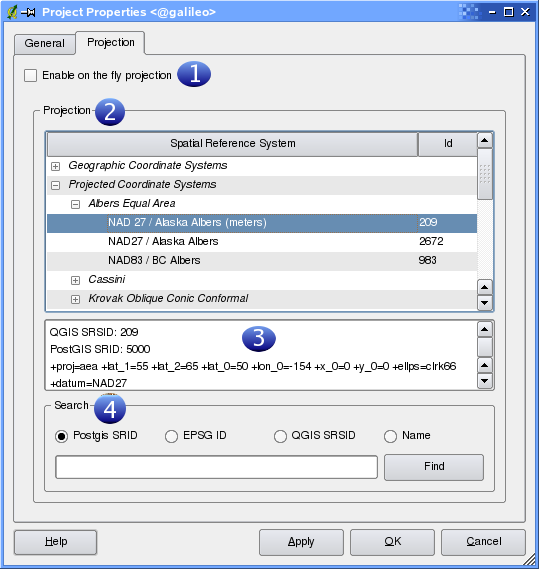
\includegraphics[clip=true, width=14cm]{projectiondialog08}
\end{center}  
\end{figure}

\begin{enumerate}
\item \textbf{Projektion zur Laufzeit einschalten}\index{Projections!enabling} -
�ber diese Checkbox wird die OTF Projektion aktiviert oder deaktiviert. Wenn sie
deaktiviert ist findet keine Projektion statt und jede Ebene wird entsprechend
der Koordinaten in der Datei dargestellt. Wenn es aktiviert ist, wird jede Ebene
beim laden in die definierte Projektion 'on-the-fly' ungewandelt dargestellt.
\item \textbf{R�umliches Referenzsystem} - dies ist eine Liste mit allen
Projektionen, die von QGIS unterst�tzt werden. Um ein Koordinatensystem zu
benutzen, w�hlt man es aus der Liste aus. Die bis dahin aktive Projektion ist vorgegeben.
\item \textbf{Proj4 Text} - dies ist ein Ausdruck, der von der PROJ-Bibliothek
genutzt wird. Es dient nur zur Information und kann nicht ver�ndert werden.
\item \textbf{Suchen} - wenn Sie die PostGIS, EPSG oder QGIS spatial\_references ID
f�r eine Projektion kennen, k�nnen Sie diese benutzen, um ihre Projektion zu
finden. Geben Sie die ID ein und klicken Sie auf \textit{Finden}.
\end{enumerate}

\subsubsection{Eine Projektion spezifizieren}
\index{Projections!specifying}
\label{sec:projection-specifying}

QGIS setzt die Projektion beim Start automatisch auf das Koordinatensystem der
ersten geladenen Ebene. Um eine Projektion zu definieren l�dt man zuerst eine
Ebene mit den gew�nschten Projektionsinformationen. Dann �ffnen Sie in der
Men�leiste unter \textit{Einstellungen}~->~\textit{Projekteinstellungen} das 
Dialogfenster \textit{Projekteigenschaften} und aktivieren im Reiter
\textit{Projektion} die Checkbox \textit{Projektion zur Laufzeit einschalten}.
Danach schlie�en Sie den Dialog und laden weitere Ebenen. 

Wenn Sie bereits einige Ebenen geladen haben und nun OTF Projektion aktivieren
m�chten, �ffnen Sie das Dialogfenster \textit{Projekteigenschaften} und w�hlen
im Reiter \textit{Projektion} die entsprechende Projektion aus der Liste. Wie
zuvor beschrieben k�nnen Sie dazu auch die Suchfunktion nutzen.  

\subsection{Eigene Projektion definieren}\label{sec:customprojections}
\index{Projections!custom}

Wenn QGIS nicht die Projektion bereith�lt, die Sie brauchen, k�nnen Sie eine
eigene Projektion erstellen. Dazu w�hlen Sie in der Men�leiste unter
\textit{Einstellungen}~->~\textit{Eigene Projektion}. Die eigene Projektion wird
in einer Benutzerdatenbank erstellt. Diese enth�lt ihre r�umlichen Lesezeichen
und die selbst erstellten Projektionen. 

\begin{figure}[ht]
   \begin{center}
   \caption{Dialog Definition einer eigenen Projektion}\label{fig:customprojections}\smallskip
   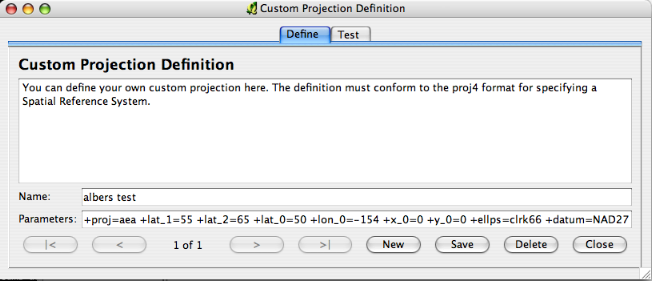
\includegraphics[clip=true, width=14cm]{customprojection}
\end{center}  
\end{figure}

In QGIS Version \CURRENT bedarf es einem grundlegenden Verst�ndnis im Umgang mit
der PROJ4-Bibliothek. Zu Beginn sollten Sie einen Blick in das Benutzerhandbuch
von PROJ werfen. Cartographic Projection Procedures for the UNIX Environment - A
User's Manual by Gerald I. Evenden, U.S. Geological Survey Open-File Report
90-284, 1990 (zu finden unter \url{ftp://ftp.remotesensing.org/proj/OF90-284.pdf}).
Dieses Handbuch beschreibt die Anwendung des Programms. Die dort beschriebenen
kartographischen Parameter sind identisch mit den in QGIS benutzten. 

Der Dialog \textit{Definition einer eigenen Projektion} braucht nur zwei
Parameter, um eine eigene Projektion zu definieren: 
\begin{enumerate}
\item Einen beschreibenden Namen
\item Die kartographischen Parameter
\end{enumerate}

Um eine neue Projektion zu erstellen, geben Sie einen beschreibenden Namen ein
und die kartographischen Parameter. Abbildung \ref{fig:customprojections} zeigt
den Dialog mit einer Beispielprojektion.

Sie k�nnen die neue Projektion testen, um zu sehen, ob bei einer Konvertierung
von bekannten WGS84 Lat-Lon Koordinaten in ihre Projektion ein sinnvolles
Ergebnis herauskommt. Klicken Sie dazu auf den Reiter \textit{Testen}, kopieren
ihre Parameter in das Feld \textit{Parameter}, geben ein paar WGS84 Lat-Lon
Koordinaten ein und klicken auf den Knopf \textit{Berechnen}. 
